\chapter{Synchronous and Parallel Approach for Offline Deduplication}
\label{chap:offline}
\section{Introduction}
\label{offline:intro}
This chapter introduces a low-cost architecture option and considers that
a backup service uses the existing cloud computing resource.
%Since most of backup data is not used in practice, system resource in such a service is not fully utilized. 
Performing deduplication adds significant  memory cost for comparison of content fingerprints. 
Since each physical machine in a cluster  hosts many VMs, memory contention happens frequently. 
Cloud providers often wish that the backup service only consumes  small or modest resources 
%with a minimal impact to the existing cloud services.  Another challenge for backup with deduplication is 
with a minimal impact to the existing cloud services.  Another challenge is 
%that deletion of old snapshots compete for computing resource as well. That is because data dependence created 
that deletion of old snapshots compete for computing resource as well, because data dependence created 
by duplicate relationship among snapshots  adds processing complexity.

The traditional approach to deduplication is an inline approach which follows
a sequence of block reading, duplicate detection,  and non-duplicate  block write to the 
backup storage. In this chapter we introduce an synchronous and parallel approach
for offline batched deduplication. This solution is suitable for cloud which typically conduct
automatic backup of all the VMs during system's spare time.
Our key idea  is to  first perform parallel duplicate detection for VM content blocks 
among all machines before performing actual data backup. Each machine
accumulates detection requests and  then performs detection   partition by partition 
with minimal resource usage.
Fingerprint based partitioning allows highly parallel duplicate detection  and also simplifies 
reference counting management.  
% as the entire process can also be divided into a
%parition-wise  deletion. 

While our synchronous offline solution accomplishes perfect deduplication efficiency while maintaining
low resource usage,
the trade-off of this approach is that the job turnaround time for each individual
VM backup task becomes longer. In addition,
every machine has to read dirty segments twice
and that some deduplication requests are delayed for staged parallel processing.
However, with our careful parallelism and buffer management,
this multi-stage detection scheme can provide a sufficient throughput for VM backup.

The rest of this chapter is organized as follows.
Section~\ref{offline:design} describes our synchronous processing steps.
Section~\ref{offline:eval} is our experimental evaluation that compares with other approaches.
Section~\ref{offline:related} reviews the related works.
Section~\ref{offline:concl} concludes this chapter.

\section{Multi-stage Synchronous Deduplication Design}
\label{offline:design}
We consider deduplication in two levels. The first level
uses coarse-grain segment  dirty bits for version-based detection~\cite{Clements2009,Vrable2009}.
% to identify difference from the previous snapshot to the current snapshot.
%That  can be accomplished efficiently and inexpensively in the OS level.
%We use a segment-level coarse-grain setting to reduce the efforts in detection and maintaining dirty bits.
Our experiment with Alibaba's production dataset shows that over 70 percentage of
duplicates can be detected using segment dirty bits when the segment size is 2M bytes.
This setting requires OS to maintain segment dirty bits and
the amount of space for this purpose is negligible. In the second level of deduplication, content blocks of dirty segments
are compared with the fingerprints of unique  blocks from the previous snapshots.
Our key strategies are explained as follows.
\begin{itemize}


\item {\bf Separation of duplicate detection and data backup.}
%Request accumulation and partition-based deduplication.}
The second level detection requires a global comparison of fingerprints.
% of stored chunks with the new chunks scanned during the backup process.
%Bloom filters and caching allows some of content
%fingerprints to be stored on the cheap disks~\cite{bottleneck08}. Such an optimization is good
%for inline deduplication where chunks scanned need to be determined to be duplicate or not instantly without
%waiting while  it memory consumption is still significant in competing with stand virtual
%machine activities.
Our approach is to perform duplicate detection first before actual data backup.
That requires a prescanning of  dirty VM segments, which
%  and after that, real backup  for those non-duplicates is conducted.
does incur an extra  round of VM reading.
% while avoiding inline deduplication and leading to a much smaller resource requirement.
During VM prescanning, detection requests are accumulated.
Aggregated deduplicate requests can be processed partition by partition.
%We also accumulate the delete requests and perform them partition by partitions.
Since each partition corresponds to a small portion of global index,
memory cost to process detection requests within a partition is small.
%the cost to process detection requests within a partition is significantly smaller than processing all
%the requests globally.

\item {\bf Buffered data redistribution in parallel duplicate detection}.
Let {\em global index} be the meta data containing the fingerprint values of unique snapshot blocks
in all VMs and  the reference pointers to the location of raw data.
%A duplicate detection request for a content block needs to be compared with the global index to determine if this
%block is non-duplicate. If it is a duplicate, return the corresponding reference pointer.
%We conduct parallel processing of detection requests in all machines involved.
A logical way to distribute detection requests among machines is based on
fingerprint values of content blocks.
% in a  disjointed manner.
Initial data  blocks follows the VM distribution
among machines
and the detected duplicate summary
should be collected following the same distribution.
Therefore, there are two all-to-all data redistribution operations involved.
One is to map detection requests from VM-based distribution to fingerprint based distribution.
Another one  is to map duplicate summary from fingerprint-based distribution to VM based distribution.
The redistributed data needs to be accumulated on the disk to reduce the use of memory.
To minimize the disk seek cost, outgoing or incoming data exchange messages are buffered to
bundle small messages.
Given there are $p\times q$ partitions where $p$ is the number of machines and $q$ is the number of fingerprint-based partitions
at each machine, space per each buffer  is small under the memory constraint for large $p$ or $q$ values.
This counteracts the effort of seek cost reduction.
%Then there will be a large number of storage  IO operations involved, suffering the huge seek overhead.
We have designed an efficient data exchange and disk data buffering  scheme to address this.

%As we detect and backup requests before actual backup takes place,  we need to store chunk data on
%temporary disks and once duplicates
%are detected, we only need to fetch and store these non-duplicates
%in the backup storage.  To minimize the storage usage of temporary disk space, we donot save the data content
%of accumulated requests with replication, but we store  data separately for each virtual machine. In an event
%that the storage of temporary accumulation fails for certain virtual machines, rescanning of these virtual machine images
%is conducted and backup of these machines is re-initiated.   Meta data such as content hash for accumulated requests
%is stored separately since we map the meta data into a set of buckets using chunk fingerprints.
%The benefit of separating content and meta data is to allow fast recovery of backup operations while enabling bucket-based lazy deduplication.

\end{itemize}

We assume a flat architecture in which  all $p$ machines that host VMs in a cluster can
be used in parallel for deduplication.
A small amount of local disk space and memory on each machine can be used
to store global index and temporary data.
The real backup storage can be either a distributed file system built on
this cluster  or use another  external storage system.
%Our design is to minimize the usage of local memory and storage on each machine.


%While we assume all machines can process  independent or coordinated
%deduplication and backup operations in parallel,
%our scheme uses a single-thread procedure on each machine to minimize the use of CPU, network bandwidth, and disk bandwidth.
We use the two level metadata hierarchy as discussed in section~\ref{overview:meta}.
The snapshot metadata  contains a list of segments and other meta data information.
Segment metadata contains its  content block fingerprints and reference pointers.
If a segment is not changed from one snapshot to another, indicated by a dirty bit embedded in the virtual disk driver,
%its content blocks are not changed as well, thus
its segment metadata contains a reference pointer to an earlier segment.
For a dirty segment, if one of its blocks is duplicate to another block in the system,
the block metadata contains a reference pointer to the earlier block.

\begin{sidewaysfigure*}[tbhp]
\centering
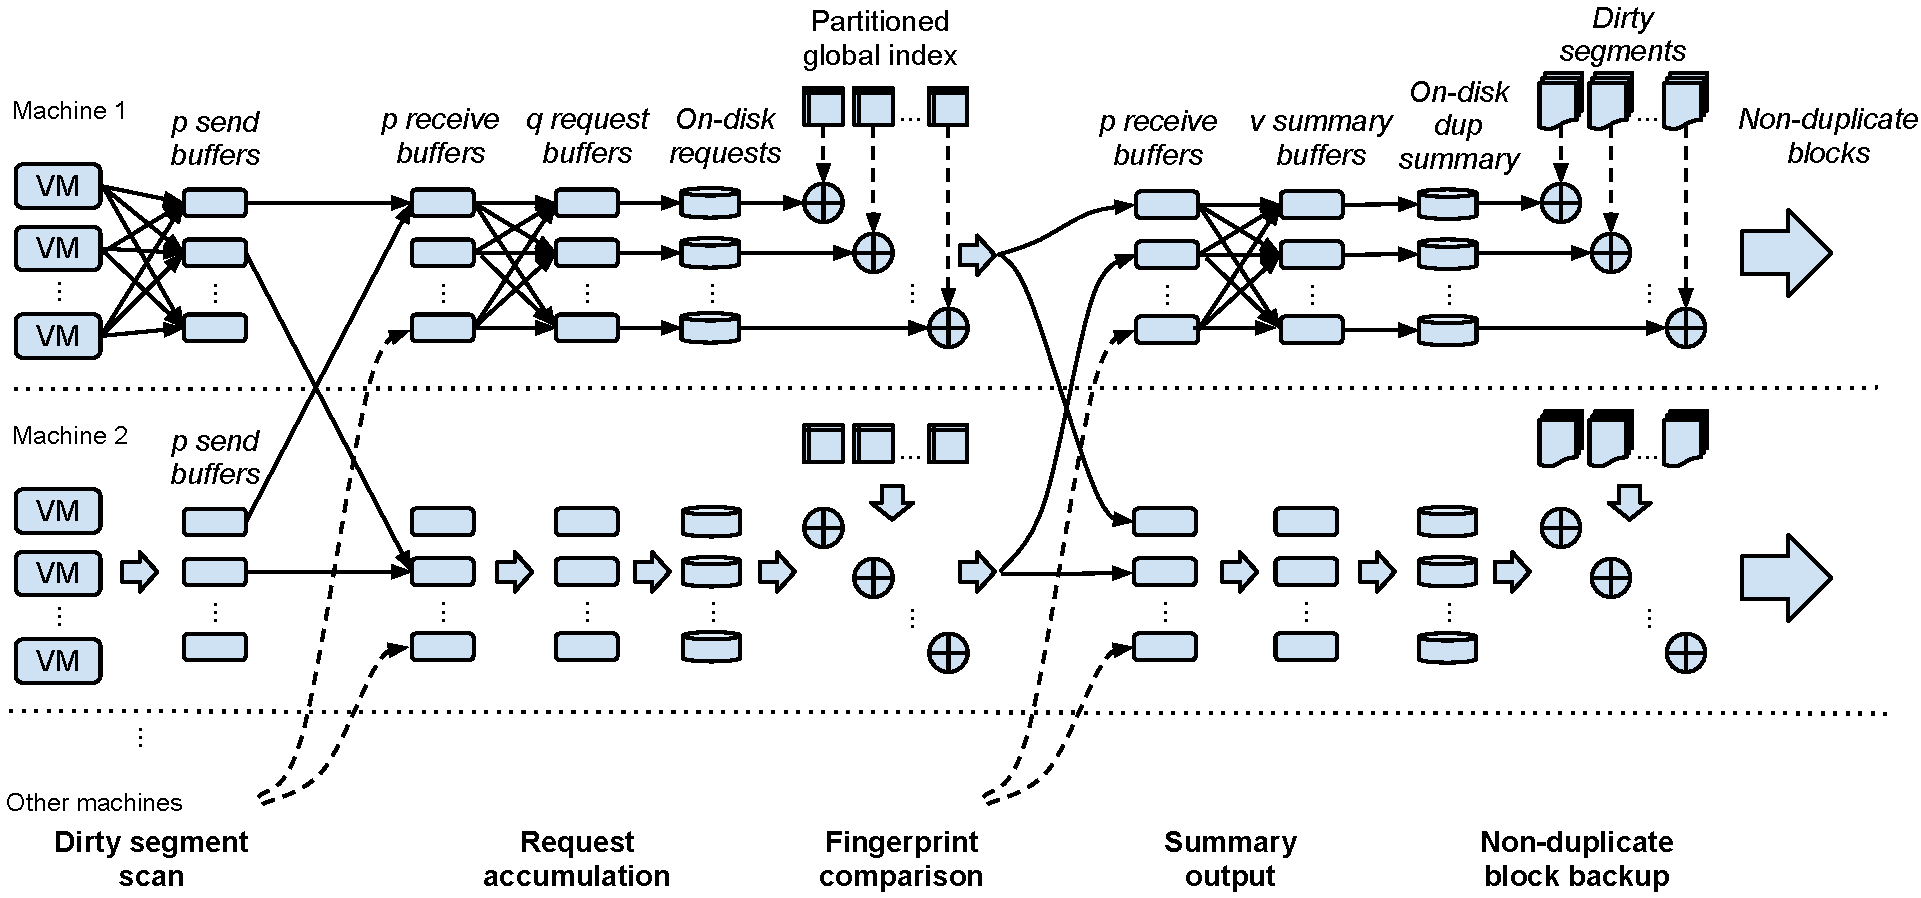
\includegraphics[height=0.45\textwidth]{images/steps.pdf}
\caption{Processing flow of Stage  1 (dirty segment scan and request accumulation), Stage 2
(fingerprint comparison and summary output),  and Stage 3 (non-duplicate block backup).}
\label{fig:flow}
\end{sidewaysfigure*}

%\subsection{Processing flow and resource usage}
The data flow of our multi-stage duplicate detection is depicted in Figure~\ref{fig:flow}.
%let $v$ be the total number of virtual machines hosted in  a cluster,
%we divide the backup into $k$  iterations.
%\begin{itemize}
%\item
In Stage 1, each machine independently reads
%$v/k$
VM images that need a backup
and forms duplicate  detection requests.
%For those dirty segments,
%segments that have been modified since last backup indicated by dirty bits,
The system divides  each dirty segment into a sequence of chunk blocks,  computes the meta
information such as chunk fingerprints,  sends a request to a proper machine, and accumulates
received requests into a partition on the local temporary disk storage.
The partition mapping uses a hash function applied to the content fingerprint.
Assuming all machines have a  homogeneous resource configuration, each machine is evenly  assigned with
$q$ partitions of global index and it accumulates corresponding requests on the disk.
There are two options to allocate buffers at each machine.
1) Each machine has  $p\times q$ send buffers corresponding to $p\times q$ partitions in the cluster
since a content block in a VM image of this machine can be sent to any of these partitions.
2) Each machine allocates $p$ send buffers to deliver requests to $p$ machines; it allocates
$p$ receive buffers to collect requests  from other machines.
Then the system copies requests from each of $p$ receive buffers to  $q$ local request buffers,
and outputs each request buffer to one of the request partitions on the disk
when this request buffer becomes full.  Option 2, which is  depicted in Figure~\ref{fig:flow},
is much more efficient than Option 1 because $2p+q$ is much smaller than
$p\times q$, except for the very small  values.
As a result, each buffer in Option 2 has a bigger size to accumulate requests and that means
less disk seek overhead.

%We assume that the startup cost for network message sending is  much more less (e.g. an order of magnitude
%less) than from one machine to another
%disk storage startup cost such as seek is much mu
%Note that we only accumulate requests with their meta data information.
%\item
Stage  2 is to load disk data and perform fingerprint comparison at each machine one request partition at a time.
% in the partitions.
%The system maintains the index of all chunk fingerprints divided in the buckets.
%The system loads the global index partition
%and accumulated corresponding requests, and compare them to  identify the duplicated blocks.
%Then we unload them, load the global index and accumulated requests for another partition.
%This process is repeated until all buckets are processed.
At each iteration, once in-memory comparison between an index partition and request partition is completed,
duplicate summary information for segments of each VM is routed from the fingerprint-based distribution  to the
VM-based distribution.  The summary contains the block ID and  the reference pointer for each detected duplicate block.
Each machine uses memory space of the request partition as a send buffer with no extra memory requirement.
But it needs to allocate $p$ receive buffers to collect duplicate summary from other machines.
It also allocates $v$ request buffers to copy duplicate summary from $p$ receive buffers and output to the local disk
when request buffers are full.

%. In this way, it sends duplicate summary to the corresponding machines one by one to minimize the startup cost for sending a message.
%In the receiving side,
%All-to-all machines data exchange is conducted  so that
%each machine allocates $q$ receive buffers corresponding to
%$q$ local partitions, to hold received messages from other machines.
%When a receive buffer for a VM is  full, the data is written to the local disk storage.
%These substeps are repeated as the stream of data is exchanged when each machine compares through all $q$ partitions.

%\item
Stage 3 is to perform real backup.
% one VM at a time.
The system loads the duplicate summary of a VM,
reads  dirty segments of a VM, and outputs non-duplicate blocks to the final backup
storage. Additionally, the global index on each machine is updated with the meta data of new chunk blocks.
When a segment is not dirty, the system only needs to output the segment meta data such as a reference pointer.
There is an option to directly read dirty blocks instead of fetching a dirty segment which can include duplicate
blocks. Our experiment shows that it is faster to read dirty segments in the tested workload.
Another issue is that during global index update after new block creation,
% in the backup storage,
the system  may find some  blocks with the same fingerprints have been
created redundantly. For example, two different VM blocks that have the same  fingerprint are not detected
because  the  global index has not contained such a fingerprint yet.
The redundancy is discovered and logged during the index update and can be repaired
periodically when necessary.  Our experience is that there is a redundancy during the initial snapshot backup and once
that is repaired, the percentage of redundant blocks due to concurrent processing  is insignificant.

%If a segment is dirty,  the system  use the duplicate summary information from Step 2 for internal
%duplicate blocks of this dirty segment and output the remaining non-duplicate blocks to the backup storage.
%\end{itemize}

%          In fetching non-duplicates,    it is sometime faster that we fetch a large number of consecutive chunk blocks from an accumulated  segment which contains duplicated chunks,  to avoid the random seek overhead.


The above steps can be executed by each machine using one thread to minimize the use of computing resource.
The  disk storage usage on each machine
is fairly small for  storing part of global index and
accumulating  duplicate detection requests that contain fingerprint information.
We impose a memory limit $M$ allocated for each stage of processing at each machine.
The usage of $M$ is controlled as follows and space allocation among buffers is optimized based on the relative
ratio between the cross-machine network  startup cost and disk access startup cost such as seek time.
Using a bigger buffer  can mitigate the impact of slower startup cost.
\begin{itemize}
\item For Stage 1, $M$  is divided for
1) an I/O buffer to read dirty segments; 2) $2p$ send/receive buffers and $q$ request  buffers.

%1) $p$ send buffers. images, sends the fingerprint of a dirty block to a machine that is responsible for this fingerprint.
%2) Buffer requests gathered from other machines and divide those requests into $q$ buckets. Once a buffer for each bucket is full, output to the disk storage.
\item
For Stage 2,  $M$  is divided for 1) space for hosting a global index partition and
the corresponding request partition; 2) $p$ receive buffers and $v$ summary buffers.
%%accumulating duplicate summary for each targeted VM.   Once  each machine processes a bucket of  duplicate detection requests,
%For each machine which hosts $v$  VMs, and will receive messages from many other machines,
%the system needs to allocate buffer space for each VM ot accumulate the duplicate summary records.
%When a buffer for a VM is full, the result is written to the disk.

\item For Stage 3, $M$  is divided for 1) an I/O buffer to read dirty segments of a VM and
write non-duplicate blocks to the  backup storage;
2) summary of duplicate blocks within dirty segments.
\end{itemize}
%We find the memory for step 2 is most critical for buffering duplicate summary in hiding the latency.
%Certainly most storage system can allow many IO requests issued in parallel overlapping the IO latency.
%Here we assume the worst case and also minimize the IO bandwidth usages by issuing
%one request at a time to use the minimal disk bandwidth resource.

{\bf Snapshot deletion.} Each VM will keep a limited number of  automatically-saved snapshots and
expired snapshots are normally deleted.
% unless its owner explicitly asks for its retention.
We adopt the idea of mark-and-sweep~\cite{Guo2011}.
A block or a segment can be deleted if its reference count is zero.
%As we discussed in Section~\ref{sect:data}, the reference counter is kept in the global index, partitioned among machines.
To delete useless  blocks or segments periodically, we read the meta data  of all
snapshots and compute the reference count of all blocks and segments  in parallel.
%while following the fingerprint-based partitioning.
Similar to the multi-stage duplicate detection process, reference counting is conducted in multi-stages.
Stage  1 is to read  the segment and block  metadata
to accumulate  reference count requests in different machines  in the fingerprint based distribution.
Stage   2 is to count references within each partition and detect those records with zero
reference.
%Stage 3 is that every VM gathers its z confirmed deletion requests for its content and sends them to the backup storage.
The backup  data repository logs deletion instructions,  and will periodically perform a compaction operation when
its deletion log is too big.


\section{System Implementation and Experimental Evaluations}
\label{offline:eval}
We have implemented and evaluated a prototype of our multi-stage deduplication scheme on a cluster
of dual quad-core Intel Nehalem 2.4GHz E5530 machines with 24GB memory.
Our implementation is based on Alibaba's Xen cloud platform~\cite{Aliyun,WeiZhangIEEE}.
Objectives of our evaluation are:
1) Analyze the deduplication throughput and effectiveness for a large number of VMs.
%Compare with the data domain approach~\cite{bottleneck08}.
2) Examine the impacts of buffering during metadata exchange.

%\subsection{Experimental setup}

%We are running our deduplication/backup  service on 100 nodes.
%Memory usage is about 150MB space per node during backup and
%the CPU usage is very small during the experiments.
We have performed a trace-driven study using  a 1323 VM dataset  collected from
%100 Alibaba Aliyun's cloud nodes~\cite{WeiZhangIEEE}.
a cloud cluster at Alibaba's Aliyun.
% ~\cite{WeiZhangIEEE}.
% and each of machine nodes has 16 cores and 12 disk drives,  hosting  up to 25 VMs.
For each VM, the system keeps 10 automatically-backed snapshots in the storage while
a user may instruct extra snapshots to be saved.
The backup of VM snapshots is completed within a few  hours every night.
Based on our study of its production  data,  each VM has about  40GB of storage  data usage on average
including OS and user data disk.
Each VM image is  divided into 2 MB fix-sized segments and each segment is divided into
variable-sized content blocks  with an average size of 4KB.
%variable sizes~\cite{similar94,rabin81} with an average size of 4KB.
The signature for variable-sized blocks is computed using their SHA-1 hash.

The seek cost of each random IO request in our test machines is about  10 milliseconds.
The average I/O usage of local storage is controlled about 50MB/second for backup
in the presence of other I/O jobs. Noted that a typical 1U server can host
6 to 8  hard drives and deliver over 300MB/second. Our setting uses 16.7\% or less
of local storage bandwidth.
The final snapshots are stored in a distributed file system built on the same
cluster.

The total local disk usage on each machine is about 8GB for the duplicate detection purpose,
mainly for global index.
Level 1 segment dirty bits identify 78\% of duplicate blocks. For the remaining dirty segments,
block-wise full deduplication removes about additional 74.5\% of duplicates.
The final content copied to the backup storage is reduced by 94.4\% in total.

\begin{figure}[htbp]
\centering
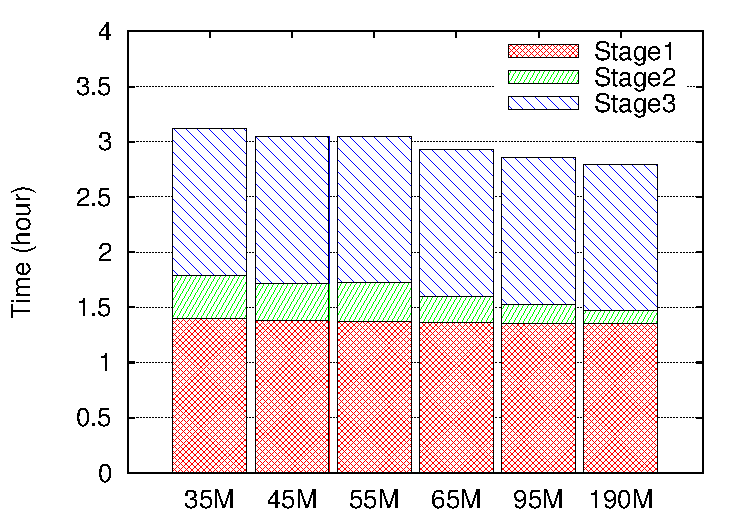
\includegraphics[width=0.6\textwidth]{figures/mem_time.pdf}
\caption{Parallel processing time when memory limit varies.}
\label{fig:memory}
\end{figure}

Figure~\ref{fig:memory} shows the total parallel time in hours to backup 2500 VMs on
 a 100-node cluster a  when
limit $M$ imposed on each node varies.
%  from 20MB to 200MB.
This figure also depicts the time breakdown for Stages 1, 2, and 3.
%The parallel time includes the first scanning time,
%of dirty VM segments to generate block fingerprints, data redistribution for request accumulation,
%fingerprint comparison, duplicate summary distribution, and the second scan time for real backup.
The time in Stages 1 and 3  is  dominated by  the two scans of dirty segments,
and final data copying to the backup storage is overlapped with VM scanning.
During dirty segment reading, the average number of consecutive dirty segments is 2.92.
%Each scan takes about 1.4 hours.
The overall processing time does not have a significant reduction as $M$ increases to 190MB.
The aggregated deduplication throughput is  about 8.76GB per second,
which is the size of 2500 VM images divided by the parallel time.
The system runs with  a single thread and  its CPU resource usage is 10-13\% of one core.
The result shows the backup with multi-stage deduplication  for all VM images can be
completed in about 3.1 hours with 35MB memory,  8GB disk overhead and a small CPU usage.
As we vary the cluster size $p$,  the parallel time does  not change much, and  the aggregated throughput
scales up linearly since the number of VMs is  $25p$.

Table~\ref{tab:overall} shows performance change when limit $M$=35MB is imposed and
the number of partitions per machine ($q$) varies.
% varies from 100 to 1000.
Row 2 is memory space required to load a partition of global index and detection requests.
When $q=100$, the required memory is 83.6 MB and this exceeds the limit $M=$35MB.
Row 3 is the parallel time and Row 4 is  the aggregated throughput of  100 nodes.
%The result shows the backup with multi-phase deduplication  for all VM images can be completed in about 3.09 hours
%with the very small resource usage.
Row 5 is  the parallel time for using Option 1 with $p\times q$ send buffers
described in Section~\ref{offline:design}.
When $q$ increases, the available space per buffer reduces and there is a big increase of seek cost.
The main network usage before performing the final data write is for request accumulation and
summary output. It lasts about 20 minutes and each machine exchanges
about   8MB of metadata per second with others during that period, which is 6.25\% of the network bandwidth.

\begin{table}[hbt]
\caption{ Performance when $M$=35MB and $q$ varies.}
\begin{center}
\begin{tabular} {|c|c|c|c|c|c|}
\hline \#Partitions ($q$)  & 100 & 250  & 500 &  750 &  1000 \\
\hline Index+request (MB) & 83.6 &  33.5 & 16.8 & 11.2 & 8.45 \\
\hline Total Time (Hours) & N/A&  3.12 & 3.15 & 3.22 & 3.29 \\
\hline Throughput (GB/s) & N/A &  8.76 & 8.67 & 8.48 & 8.30 \\
\hline Total time (Option 1) & N/A&  7.8& 11.7 & 14.8 & 26 \\
\hline
\end{tabular}
\end{center}
\label{tab:overall}
\end{table}


\section{Related Work}
\label{offline:related}
%In a virtualized cloud environment such as ones provided by Amazon EC2\cite{AmazonEC2} and Alibaba Aliyun\cite{Aliyun},
At a cloud cluster node, each instance of a guest operating system runs on a virtual machine, accessing virtual hard disks
represented as virtual disk image files in the host operating system.
For VM snapshot backup, file-level semantics are normally not provided.
Snapshot operations take place at the virtual device driver level, which means no fine-grained file system metadata can be used to determine the changed data.
%Only raw access information at disk block level are provided.
%Each physical machine hosts many VMs and petabytes of data in a cloud cluster need a frequent  backup.
%Ideally speaking, snapshot backup must not affect the normal cloud service, which means that
%only a very small slice of cluster resource can be used for the backup purpose.

%The previous work for storage backup has extensively used  data deduplication techniques can eliminate redundancy globally among different files from different users.
Backup systems have been developed to use content fingerprints to identify duplicate
content~\cite{venti02,Rhea2008}.
Offline deduplication is
used in ~\cite{EMC,NetAppOffline} to remove previously written duplicate blocks during idle time.
%,NGmiddleware2011}.
%Today's commercial data backup systems (e.g. from EMC and NetApp)
%\cite{emc_avamar}\cite{datadomain_whitepaper}
%use a variable-size chunking algorithm to detect duplicates in file data~\cite{similar94,hydrastor09}.
Several techniques have been proposed to speedup searching of duplicate
fingerprints. For example, the data domain method ~\cite{bottleneck08}
uses  an in-memory Bloom filter and a prefetching cache for data blocks  which may be
accessed.  An improvement to this work with parallelization is in ~\cite{MAD210,DEBAR}.
As discussed in Section~\ref{offline:intro},
there is no dedicated resource for deduplication in our targeted setting and low memory usage
 is required so that the resource impact to other cloud services is minimized.
%NG et al.~\cite{ NGmiddleware2011}  use
%a related filtering technique for integrating deduplication in Linux  file system and the memory
%consumed is up to 2GB for a single machine. That is still too big in our context discussed below.
%Lillibridge et al.~\cite{sparseindex09} break list of chunks
%into large segments, the chunk IDs in each incoming segment are sampled and the segment is
%deduplicated by comparing with the chunk IDs of only a few carefully selected backed up segments.
%These are segments that share many chunk IDs with the incoming segment with high probability.
The approximation techniques are studied in~\cite{extreme_binning09,Guo2011}
%Deepavali et al.~\cite{extreme_binning09} and Zhang et al.~\cite{WeiZhangIEEE}
to reduce memory requirement with a trade-off of the reduced deduplication ratio.
%use fingerprint-based file similarity  and group similar files into the same physical location (bins) to deduplicate against each other.
%That leads  to a smaller amount of memory usage for storing meta data in fingerprint
%lookup
In comparison, this paper focuses on  full deduplication without approximation.
%We also take advantages of the fact that in a VM cloud environment,
%the virtual device driver can easily keep track if  large data
%segments have been modified using dirty bits and such information can avoid sending
%unmodified data segments for deduplication, which significantly saves cost.

Additional inline deduplication techniques are studied in ~\cite{sparseindex09,Guo2011,Srinivasan2012}.
All of the above approaches have focused on
such inline duplicate detection in which  deduplication of an individual block  is on the critical write path.
In our work, this constraint is relaxed and
there is a waiting time for many duplicate detection requests. This relaxation is acceptable because
in our context, finishing the backup of required VM images within a reasonable time window is more
important than optimizing individual VM block  backup requests.

\section{Concluding Remarks}
\label{offline:concl}
The contribution  of this work is a low-cost multi-stage parallel deduplication solution.
Because of separation  of duplicate detection and actual backup,
we are able to evenly distribute  fingerprint comparison among clustered machine
nodes, and only load one partition at time at each machine for in-memory comparison.
%The trade-off is that every machine has to read dirty segments twice
%and that some deduplication requests are delayed for staged processing.  

The proposed  scheme is resource-friendly to the existing cloud services.
The evaluation shows that the overall 
deduplication time and throughput of 100 machines  are satisfactory with 
about 8.76GB per second for 2500 VMs. During processing, each machine uses 
35MB memory, 8GB disk space, and 10-13\% of one CPU core with a single thread  execution.
Our future work is to conduct more experiments with production workloads.
%and a modest use of IO and network resource.
%Thus the proposed  scheme does not take a significant  amount of the resource away
%to compete with the existing cloud services.
%While using an insignificant system resource,
%When the cluster size changes, our experiment also shows a linear speedup of overall throughputs
%because highly parallel fingerprint comparisons.  
%The cluster  of 100 nodes and 2500 VMs can deliver about 
%8.8GB per second deduplication performance.  We expect the system performs well in a larger cloud 
%setting and 

The major limitation of our synchronous approach is that all VM snapshots must be processed together
in order to achieve maximum aggregated throughput, as a result, small VMs need to wait big VMs during
the duplicate detection phase until all VMs finishes stage 2. Since the small VM disks 
need to be put under copy-on-write protection longer, their disk I/O performance will be slow down
and  additional disk space are needed to store the modified segments during backup. Another limitation
is that VM user cannot choose the time of taking snapshot freely. Therefore, our synchronous approach 
is ideal for private cloud in which the IT admin needs to backup all the VMs together, but it may not
be suitable 
for public cloud which demands real-time snapshot backup operation. We will discuss our solution
for on demand inline deduplication in the next chapter.

